




\section{Speicher-Hierarchie}

\begin{figure}[htbp]

	\begin{minipage}{0.5\textwidth}		
		\begin{itemize}[noitemsep,topsep=0pt]
			\item Speicher nahe an CPU $\rightarrow$ hohe Speicherperformance (kurze Zugriffszeiten) gefordert
			\item Forderung an Speicher: schnelle Zugriffszeiten, minimale Kosten
			\item Rechner benutzen deshalb oft hierarchisch organisierten Speicher. Die Anzahl an Hierarchiestufen kann von Rechner zu Rechner start variieren.
		\end{itemize}
        \begin{itemize}
        \item hirarchische Organisazion der Bussysteme und Systemspeicher
        \item Caches
        \item Adresstransformation
        \item Multiprozessorstruktur
        \item Systemkomponenten 
    \end{itemize}	
	\end{minipage}
	\hfill		
	\begin{minipage}{0.45\textwidth} 
		\includegraphics[width=\textwidth]{images/Speicherhierarchie/UebersichtSpeicherhierarchie.PNG}
	\end{minipage}
	
\end{figure}
Zwischen L1 \& L2 ist ein Interface zum Hauptspeicher und zu externen Systemkomponenten
\begin{itemize}
    \item kommuniziert auch mit L2 und In/Outputs
    \item Busbreite häufig das doppelte der Prozessor-Wortbreite
\end{itemize}
\begin{minipage}{\linewidth}
    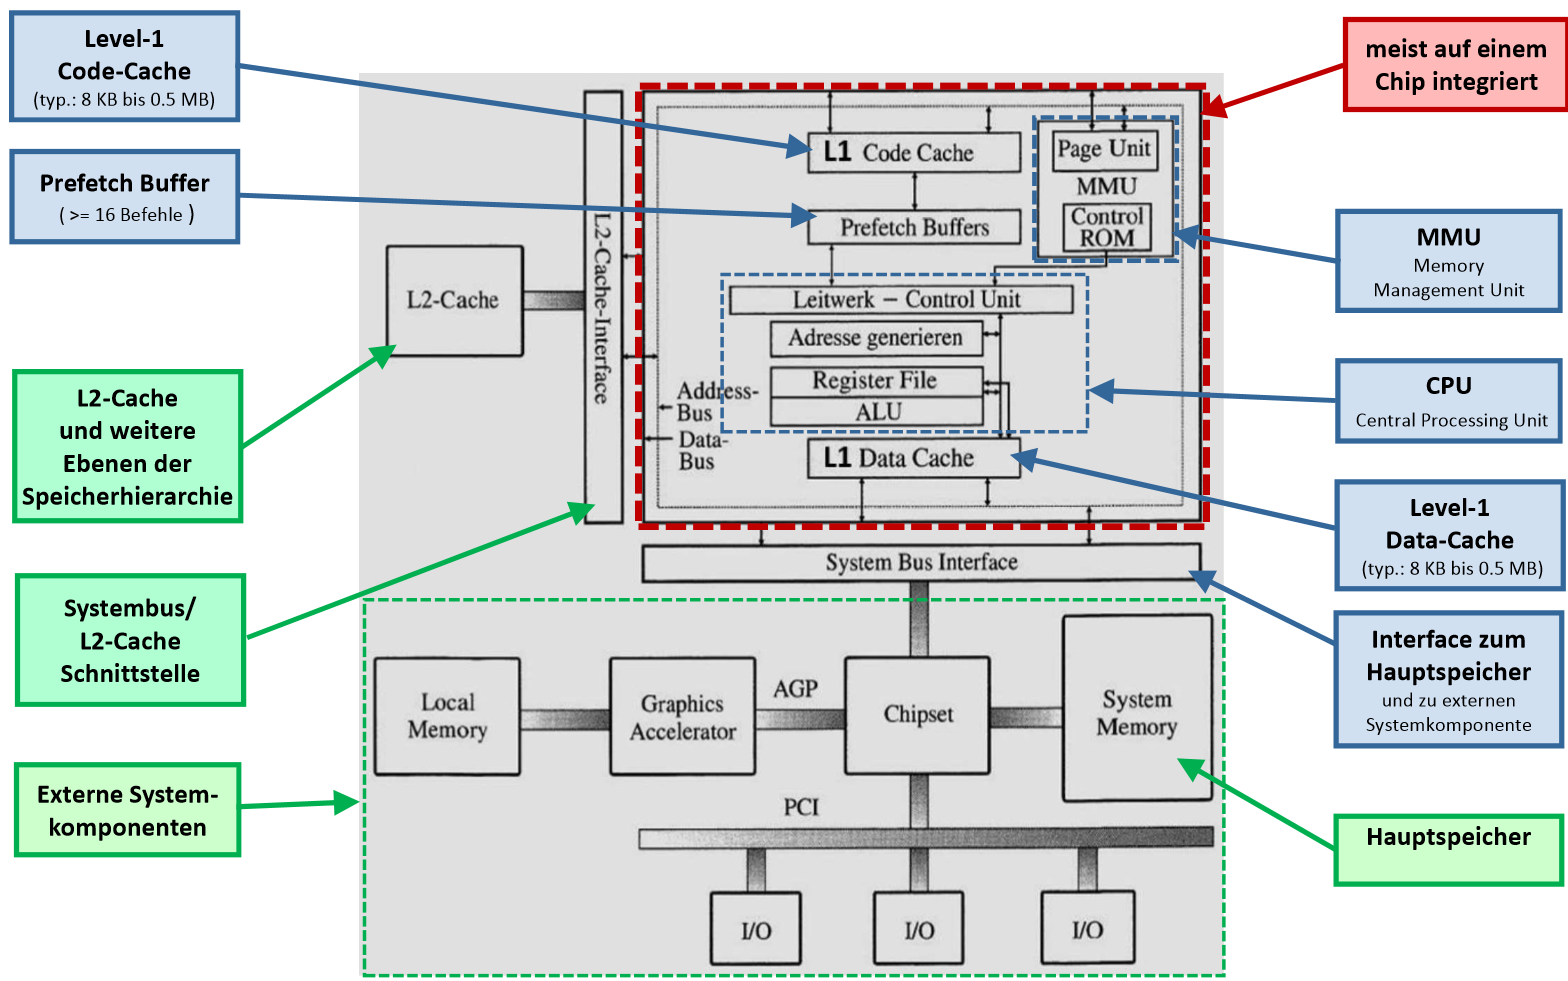
\includegraphics[width=0.7\textwidth]{images/SystembusSpeicherSpeichersystem/SpeicherSysStrukt}\centering
\end{minipage}\newline


\subsubsection{Systembus}
Der Systembus (auch CPU-, Prozessor- oder Host-Bus gennant) ist der Bus, über den die CPU mit ihrer direkten Umgebung, also insbesondere mit dem L2-Cache, dem Hauptspeicher und den Ein/Augabe-Ports kommuniziert.\newline
\textbf{Bei Übertragungsraten gilt normalerweise: 1MByte/s = $ 10^6 $Bytes/s (nicht $ 2^{20}$ Bytes/s)}\newline
\vspace{-0.5cm}
\subsubsection{Einzel vs Burst-Transfer}
    \begin{minipage}{0.5\linewidth}
        \textbf{Einzel-Transfer}
        \begin{itemize}
            \item Transfer von/zu Speichersystem, Register, I/O-Geräte
            \item Datengrösse
            \subitem 1..8 Byte
            \subitem 2 Takte
            \item  *CACHE = inaktiv
        \end{itemize}
    \end{minipage}   
    \begin{minipage}{0.5\linewidth}
        \textbf{Burst-Transfer (Block Transer)}
        \begin{itemize}
            \item Nach dem ersten Clock werdeb bei jedem weitereb Clock Dateb übertragen
            \item Die Adreaae wird im Speichersystem selber erzeugt
            \item Pentium
            \subitem 4 Pakete a 64 Bit $ \rightarrow $ 32 Byte
            \subitem 2 - 1 - 1 - 1 $ \rightarrow $ 5 Takte
        \end{itemize}
    \end{minipage}

\subsection{Leistungsmasse unf Anforderungen}
\subsubsection{Speicherbandbreite}
Anzahl Bit/Bytes, die in einer Zeiteinheit transferiert werden können.\newline
\begin{tabular}{cl}
    $ S_p = L_p \cdot SB_p $&$ S_p $= Speicherbandbreite in byte/s\\
    & $ L_p $= Leistung eines Prozessors P in MIPS (Millionen Instruktionen pro Sekunde)\\
    &$ SB_p $= Speicherbedarf (in Byte) pro Durchschnittsbefel des Prozessors P\\   
\end{tabular}\newline
Intensive Nutzung von Load/Store-Befehlen, wie dies bei RISC-Architecturen typisch ist, erhöht sich der $ SB_P $ deutlich.

\subsubsection{Prozessor-Leistung}
\begin{tabular}{cl}
    $ L_p = \dfrac{1}{CPI_p \cdot T_p} $ & $ L_p $= Leistung eines Prozessors P in MIPS (Millionen Instruktionen pro Sekunde)\\
    &$ T_p $= Taktzyklus des Prozessors in $ \mu $s\\
    &$ CPI_p $= Zahl der Taktzyklen pro Durchschnittsbefehl des Prozessors P ( Cycles per Instruction)\\   
\end{tabular}
Der $ CPI_p $ kann statistisch oder abhängig von bestimmten Programmen ermittelt werden. Da heutige Prozessoren oft superskalar implementiert sind, werden $ CPI_p $-Werte von unter 1.0 erreicht.

%----------------------------------------------------------------------------------------------
\subsection{Lokalitätsprinzip}

Idee: Innerhalb grösserer Zeiträume wird nur ein Teil des gesamten Codeumfangs ausgeführt (Programm bleibt in ähnlichem Adressbereich z.B. bei Schleifen).
Die Speicherzugriffe in dieser Zeit bezeichnet man auch als Working Set $W(t-T,t)$.
\textbf{Der Working Set $W(t-T,t)$ bleibt für grössere Zeiträume unverändert.}

\begin{figure}[ht]
	\begin{minipage}[t]{0.475\textwidth}
		\textbf{Räumliche Lokalität (spatial locality)}\\
		Wird auf eine bestimmte Adresse im Hauptspeicher zugegriffen, so ist die Wahrscheinlichkeit relativ hoch, dass der folgende Zugriff auf eine Adresse in der Nachberschaft geht (z.B. bei Schleifen).
		In Speichersystem werden adressmässig benachbarte Bytes zusammen zu höheren Ebenen der Hierarchie verschoben.
	\end{minipage}
	\hfill
	\begin{minipage}[t]{0.475\textwidth}
		\textbf{Zeitliche Lokalität (temporal locality)}\\
		Wird auf eine bestimmt Adresse im Hauptspeicher zugegriffen, so ist die Wahrscheinlichkeit relativ hoch, dass in naher Zukunft wieder darauf zugegriffen wird (z.B. Verwendung einer Variable).
		Diese Daten werden auf der schnellsten Stufe der Hierarchie gehalten.
	\end{minipage}	
\end{figure}

%----------------------------------------------------------------------------------------------
\subsection{Cache-Speicher}

\subsubsection{Aufbau und Übersicht}
Der Cache ist ein schneller Zwischenspeicher, der innerhalb der CPU selbst oder in unmittelbarer nähe angeordnet ist.
Er enthählt Daten und/oder Instruktionen, auf die in einem bestimmten Zeitraum zugegriffen werden muss (Lokalitätsprinzip).

\begin{figure}[htbp]
	
	\begin{minipage}{0.5\textwidth}		
		\begin{itemize}[noitemsep,topsep=0pt]
			\item Jeder Cache besteht aus einem Daten-Bereich und einem Tag-Bereich.
			\item Datenbereich ist normalerweise deutlich kleiner.
			\item Tag-Bereich enthält Teil der CPU-Adresse, womit Herkunft eines Cache-Eintrags aus Hauptspeicher eindeutig identifiziert werden kann.
			\item Folgende Punkte sind bei jedem Cache festzulegen: \textbf{strukturelle Parameter}, \textbf{Organisationsform} und die \textbf{Ersetzungsstrategie}
		\end{itemize}	
	\end{minipage}
	\hfill		
	\begin{minipage}{0.45\textwidth} 
		\includegraphics[width=\textwidth]{images/Speicherhierarchie/GrundstrukturCache.PNG}
	\end{minipage}
	
\end{figure}

\subsubsection{Cache-Hierarchie}
Oftmals sind mehrere Caches vorhanden. Level 1 Cache (L1-Chache) ist innerhalb CPU angeordnet und arbeitet mit der CPU-Geschwindigkeit.
Er benötigt grossteil der Chipfläche und ist bis ca. $128 \ kByte$ beschränkt.\\
L2-, L3-Cache sind meistens ausserhalb der CPU angeordnet und sind wesentlich langsamer als L1-Cache.
Greift man auf diese zu entstehen Wait-States. Grösse ist typischerweise 256 kByte bis mehrere MByte. \newline 

Die Cache-Lines haben eine einheitliche Grösse von $2^i$ Bytes.
Die Blocknummer (Tag) kann direkt aus dem Bitmuster der Hauptspeicheradresse abgeleitet werden:
\begin{equation*}
	Blocknummer = Hauptspeicheradresse \ DIV \ 2^i
\end{equation*}

\begin{equation*}
	Cache-Gr\ddot{o}sse = 2^{k+i}
\end{equation*}

Bei der Cache-Aktualisierung werden immer $2^i$ Bytes übertragen (Burst-Modus).
Zudem muss überprüft werden, ob die Information bereits im Cache vorahnden ist.
Folgende Schritte sind notwendig:
\begin{enumerate}[noitemsep,topsep=0pt]
	\item Blocknummer bestimmen (Speicheradresse DIV $2^i$)
	\item Gesuchten Blocknummer bei gültigen Einträgen vergleichen (CAM-Speicher)
	\item Wenn gefunden (Cache-Hit): Daten aus Cache-Zeile extrahieren und Prozessor übergeben (Zugriff beendet)
	\item Falls nicht gefunden (Cache-Miss):
	\begin{enumerate}[noitemsep,topsep=0pt]
		\item Ganze Cache-Zeile aus Hauptspeicher in Cache nachladen, Tag-Eintrag und Valid-Flag setzen.
		\item Gesuchte Daten aus Cache-Zeile extrahieren und Prozessor übergeben
	\end{enumerate}
\end{enumerate}

	\textbf{Voll-Assioziative Cache-Organisation}
	\begin{itemize}[noitemsep,topsep=0pt]
		\item Gesuchte Dateneinheit kann an beliebiger Stelle im Cache sein.
		\item bei CAM-Zugriff sind $2 ^k$ Vergleiche notwenig. Bei grossen Cache-Speichern deshalb langsam
	\end{itemize}

	\textbf{Einweg-Assioziative Cache-Organisation}
	\begin{itemize}[noitemsep,topsep=0pt]
		\item Eindeutige Abbildung zwischen Blocknummern und Cache-Zeilennummern, deshalb nur ein Adressvergleich notwendig
		\item Adresseintrag (Tag) verkürzt sich um $k$
		\item Bei einer ungünstigen Folge von Speicherzugriffen kann sehr häufiges Nachladen erforderlich sein.
	\end{itemize}
	\begin{align*}
		Zeilennummer &= Blocknummer \ MOD \ 2^k\\
		Adresseintrag &= Blocknummer \ DIV \ 2^k
	\end{align*}

%todo{n-Weg assoziative Oranisation ergänzen, alles hier etwas unklar.}

\subsubsection{Cache-Ersetzungsstrategien}
%{\large{\textbf{Cache-Ersetzungsstrategien}}}\\
	\begin{itemize}[noitemsep,topsep=0pt]
		\item Least Recenty Used Algorithmus (LRU):\\
		Der am längsten nicht benutzte Eintrag wird ausgewählt und ersetzt
		\item Random Strategie:\\
		Es wird ein zufälliger (oder pseudozufälliger) Eintrag ausgewählt und ersetzt
		\item Least Fequently Used Algorithmus:\\
		Der am wenigsten oft verwendete Eintrag wird ausgewählt und ersetzt.
		\item Pseudo-LRU:\\
		Echte LRU-Algorithmen sind aufwändig in Umsetzung, oftmals deshalb Pseudo-LRU (werden z.B. mit Vergangenheitsbits realisiert, Vergangenheitsbits werden bei jeder Benutzung des Blocks aktualisiert.
		Eine Logik entscheidet, welcher Block überschrieben werden soll.)
	\end{itemize}
	
	\subsubsection{Cache-Performance}
%{\large{\textbf{Cache-Performance}}}\\
Die Cache-Konfiguration hat einen wesentlichen Einfluss auf die Performance.
Normalerweise gilt jedoch: Je grösser der Cache, desto höher die zu erwartende Perfomance.

\textbf{Durchschnittliche Zugriffszeit}\\
Bei gemeinsamen Caches für Daten und Befehle ist mit einer grossen Anzahl Nicht-Treffern zu rechnen.
Je nach Grösse macht es deshalb Sinn getrennte Caches einzusetzen. Die durchschnittliche Zugriffszeit ergibt sich aus der Zugriffszeit auf den Cache $T_{eff}$, der Miss-Rate $r_{Miss}$ [\%] und der Zusatzzeitaufwand bei Miss $A_{Miss}$.
\begin{equation*}
	\mathrm{Durchschnittliche \ Zugriffszeit:} \qquad T_{eff} = T_{Hit} + r_{Miss} \cdot A_{Miss}
\end{equation*}

\begin{equation*}
\mathrm{Mit \ L2-Cache:} \qquad T_{eff} = T_{Hit-L1} + r_{Miss-L1} \cdot \left( T_{Hit-L2} + r_{Miss-L2} \cdot A_{Miss-L2} \right)
\end{equation*}

\textbf{Cache-Stragegien}
\begin{itemize}[noitemsep,topsep=0pt]
	\item Write Through (Store Through)-Strategie:\\
	Daten werden bei jedem Schreibzyklus in den Hauptspeicher zurückgeschrieben (ev. hat es auch einen Schreibpuffer).
	Die Daten sind dadurch im Hauptspeicher immer konsistent, jedoch gibt es ev. viele unnötige Schreiboperationen.
	Bei Mehrprozessorsystemen gibt es keine Cache-Kohärenz.
	
	\item Write Back (Copyback, Store In)-Strategie:\\
	Bei einem Cache-Treffer wird der Cache-Inhalt aktualisiert und ein Modified-Flag bei dem Eintrag gesetzt.
	Wert wird später in Hauptspeicher zurückgeschrieben (durch Maschineninstruktion, Hardware-Signal).
	
	\item Write Allocate (Copyback Store In)-Strategie:
\end{itemize}

\textbf{Zu beachten}
\begin{itemize}[noitemsep,topsep=0pt]
	\item Der Peripherie-Adressraum (bzw. I/O-Bereiche) darf niemals über Cache bedient werden, da sonst eine wiederholte Statusabfrage eines Peripherieregisters immer dieselbe Information liefern würde.
	
	\item Der Cache-Speicher beschleunigt lediglich den Zugriff auf den Speicher.
	
\end{itemize}

\subsubsection{Cache-Kohärenz}
%{\large{\textbf{Cache-Kohärenz}}}\\
Die Cache-Kohärenz ist eine Eigenschaft von Systemen, bei denen sich mehrere Prozessoren und/oder Controller, welche zumindest teilweise über Caches verfügen, einen gemeinsamen Haupspeicher teilen.
Cache-Kohärenz liegt dann vor, wenn jede Veränderung an gemeinsam genutzten Daten rechtzeitig den andern Nutern mitgeteilt wird.
In Einprozessor-Systemen entstehen auch Kohärenzprobleme, wenn mehrstufige Caches implementiert sind.

\textbf{Lösungsansätze}
\begin{itemize}[noitemsep,topsep=0pt]
	\item Geimeinsame Daten werden nicht über Cache geführt (ergibt Geschwindigkeitsverlust)
	\item Alle Caches arbeiten nach der Write Through-Strategie\\
	Jeder Cash-Kontroller überwacht Zugriffe der anderen Master (Snooping). Sobald ein anderer Cache auf Daten zugreift die in diesem Cache vorhanden sind, wird das Valid-Bit gelöscht.
	\item Für alle Cache-Strategien ist die Anwendung eines Kohärenzprotokolls möglich.\\
	Hierbei beobachten die einzelnen Cache, Kontroller ebenfalls den Bus, können aber zusätzlich noch Informationen untereinander austauschen. Diese sind Modified, Exclusive, Shared, und Invalid (MESI-Protokoll).
\end{itemize}
%\todo{Letzte Seiten überprüfen und ergänzen}